\documentclass{standalone}
\usepackage[spanish]{babel}   %%para Colocar en Español
\usepackage[latin5]{inputenc} %%para usar tildes adecuadamente

\begin{document}
	\section*{Marco te\'orico}
	Ejemplo para realizar citaciones dentro del documento: Se pueden citar referencias ualeindivids \cite{murphy} o tambi�n se pueden citar m�ltiples referencias \cite{murphy,matlab}. 
	
	Ejemplo para usar figuras: En la Figura \ref{fig:stoxs_2016} se observan  3 robots del equipo STOx's en partido oficial de RoboCup 2016.
	
	\begin{figure}
		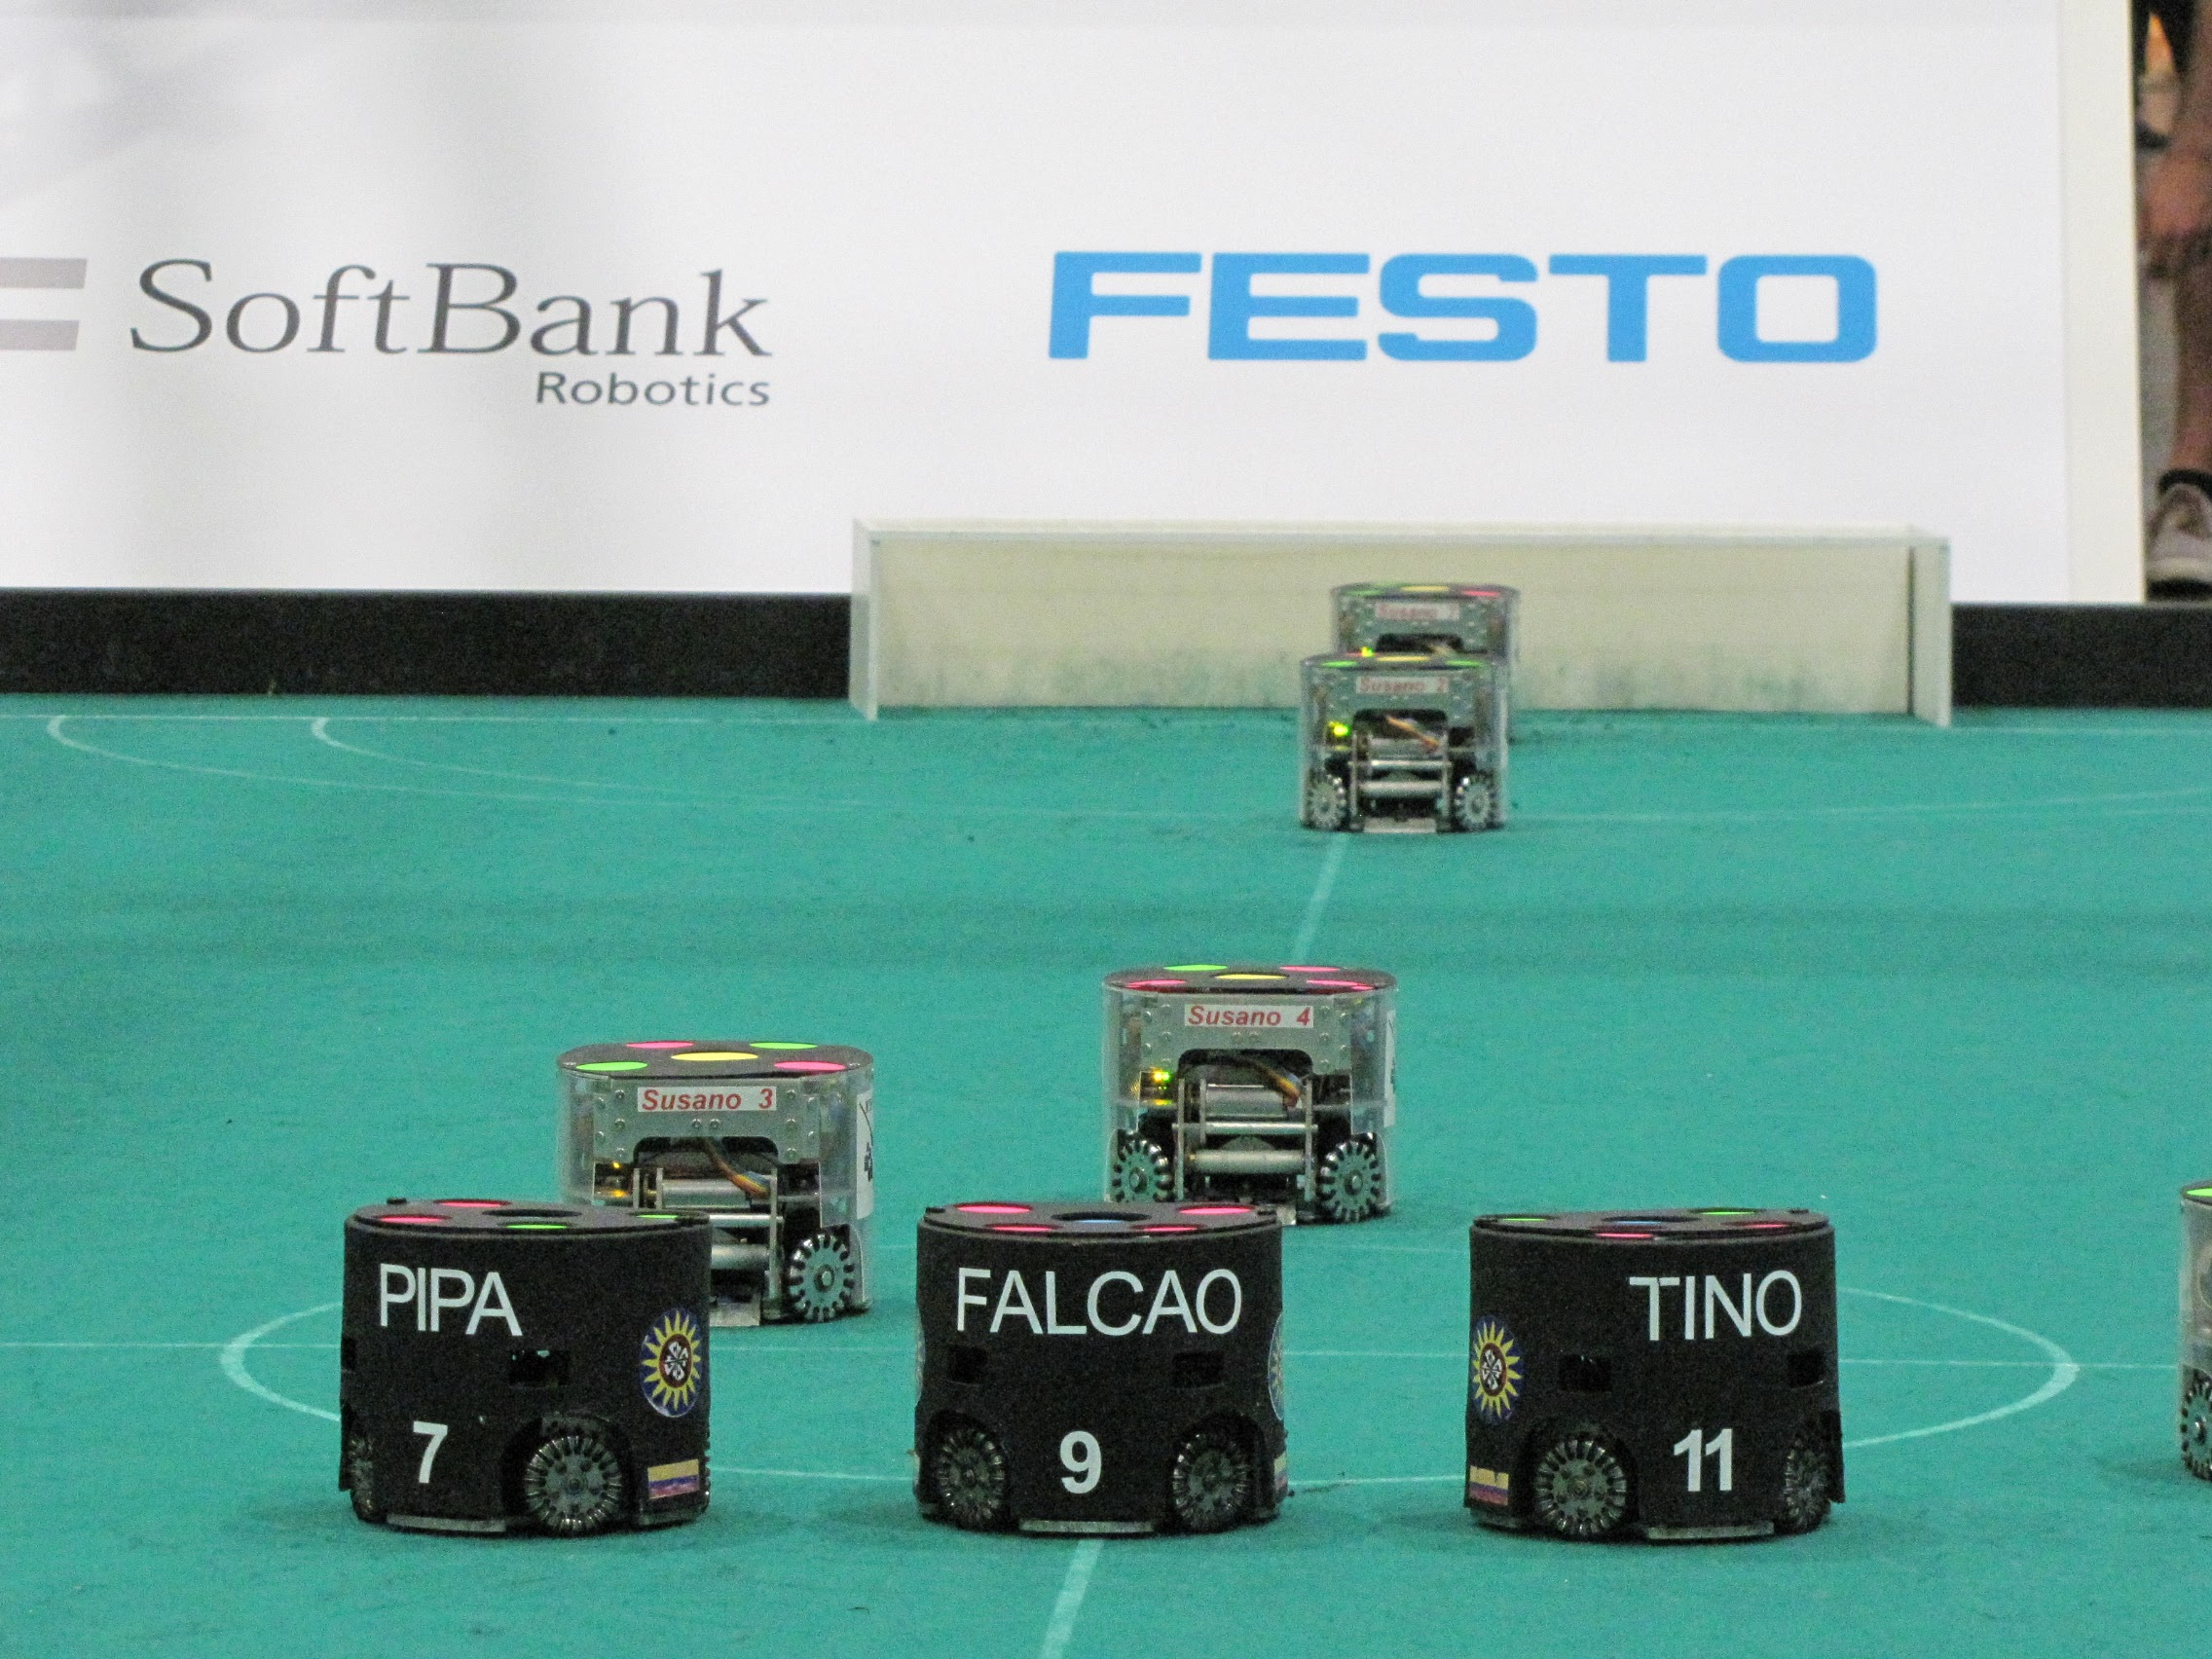
\includegraphics[width=\textwidth]{STOxs.jpg}
		\caption{Robots del equipo STOx's en RoboCup 2016}
		\label{fig:stoxs_2016}
	\end{figure}

\end{document}